\paragraph{}En esta página se puede observar el listado completo de todos los microcontroladores existentes en el catálogo electronico. En la parte derecha de la tabla, tras la especificación de cada microcontrolador, se hallan los siguientes botones:
\begin{itemize}
	\item \textbf{Editar:} Redirige al administrador a la página para editar la especificación y características de dicho microcontrolador.
	\item \textbf{Eliminar:} Elimina el microcontrolador de la base de datos del catálogo electrónico, recargando la página con el nuevo listado actualizado.
\end{itemize}

\begin{figure}[h!]
	\centering
	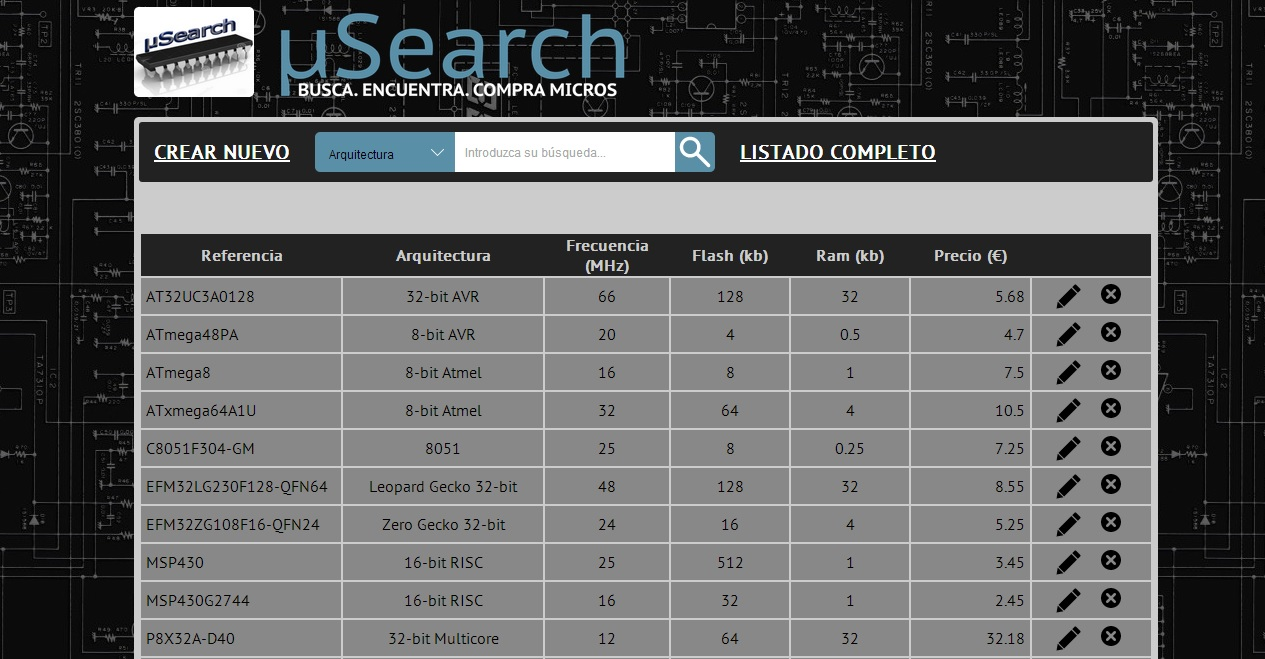
\includegraphics[width=0.80\textwidth]{img/listado_completo_admin}
	\caption{Página de listado completo de micro-controladores.}
	\label{fig:listado_completo_admin}
\end{figure}

\paragraph{}Desde esta página, a través de los iconos situados en la cabecera debajo de los logotipos de la web, el administrador puede acceder a:

\begin{itemize}
	
	\item \textbf{Crear Nuevo:} Redirige al administrador a la página para añadir un nuevo microcontrolador al catálogo electrónico.
		
	\item \textbf{Búsqueda:} Desde esta sección, el administrador puede realizar búsquedas sobre el catálogo de microcontroladores en base a cualquiera de sus características (Arquitectura, Frecuencia, Flash, RAM). Se debe seleccionar una de las características de la lista despegable, introducir el texto a buscar y pulsar sobre el icono de búsqueda.
	El usuario será redirigido a una página donde se le mostrará el resultado de la búsqueda.
			
	\item \textbf{Listado Completo:} Recarga la página actual.
\end{itemize}